% Chapter 4
\chapter{Conception}

\label{Chapter4} 
le Software-Defined Networking a rapidement émergé comme une technologie prometteuse pour les réseaux futurs et a gagné beaucoup d'attention. Cependant, la nature centralisée du SDN rend le système vulnérable aux attaques par déni de service (Dos), une fois le contrôleur compris, tout le réseau cessera de fonctionner. Mais cette centralisation a un avantage, la gestion centralisée des équipements réseau, elle permet d'avoir une vue globale des flux de trafic, ce qui offre un meilleur système de défense contre les attaques DoS.\\

Comme mentionné dans la section \ref{rDoS}, nous nous intéressons dans notre travail à une attaque DOS spécifique, connue sous le nom de \textbf{Reflective-DoS} (RDos). Cette attaque est un peu spéciale et diffère carrément des autres types d'attaques Dos, dans le principe de fonctionnement et les dommages causés. On parlera plus sur cette attaque dans la section suivante. \\

Ce chapitre portera sur la conception de notre solution. Nous commençons par la problématique et la motivation de notre travail, suivi des hypothèses de conception. On passera après à la première étape de la conception, où on présentera l'architecture de notre système et ses différents composants. L'étape suivante est la construction de notre modèle de clustering  et terminera évidemment avec une conclusion sur le travail effectué.

\section{Problématique}
Mars 2018, un nouveau record a été marqué avec 1.7 Tbps de trafic généré par une attaque DoS réflective. La compagnie \textbf{Arbor Networks} a affirmé que son système d'analyse de trafic, ATLAS, a enregistré 1.7 Tbps d'une attaque reflective contre un site web d'un client[\cite{19}].\\

RDoS n’attaque pas directement la cible mais envoie plutôt plusieurs requêtes vers un service tiers exploitable (c. -à-d. le réflecteur, généralement c'est un serveur) avec une adresse IP d’expéditeur usurpée, ce qui rend l'attaquant anonymat. Les réponses du serveur tiers sont ensuite envoyées à la cible d’attaque réelle et causer une surcharge. Les protocoles avec des messages de réponse qui sont beaucoup plus grands que les messages de demande sont particulièrement bien adapté à ces attaques en raison des effets d’amplification. La nature de ces attaques nécessite des services qui fonctionnent sans connexion établie entre le client et le serveur. Une étude récente[\cite{20}] a trouvé que $ 99.72\% $ des attauqes RDoS utilisent des protocols basé UDP, comme DNS, NTP, ..etc. Les messages reçus dans une attaque RDoS sont difficiles à différencier du trafic bénin, car ils sont conformes aux spécifications du protocole. Les réflecteurs sont correctement gèrent toutes les demandes comme légitimes, mais l’absence de réponse est une caractéristique des attaques réflectives qui ne peut être masquée.

\begin{figure}[h]
\centering
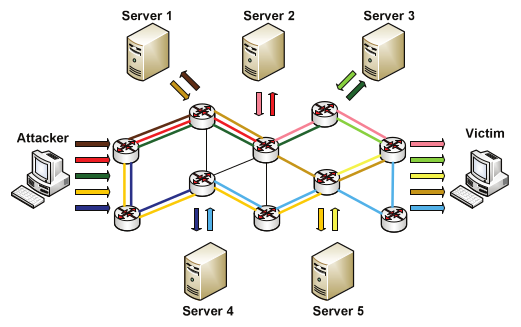
\includegraphics[width=0.7\textwidth]{Figures/rDoS}
\decoRule
\caption{Principe de dénie de service réflectif}
\label{fig:rDoS}
\end{figure} 

À ce niveau, on peut clairement voir que l'impact de ce type d'attaque est en double; en premier lieu, la consommation de la bande passante des liens réseau à cause au nombre excessive des messages requêtes et réponses échangés. En deuxième lieu, la surchage des serveurs tiers avec des messages requêtes, qui vont les traiter évidemment, car pour eux ils paraissent des requêtes légitimes.\\ 

\section{Motivation du travail}
Un article[\cite{21}] sur les travaux connexes a montré que la défense contre les attaques RDoS peut être divisée en 3 principales tâches : (1) surveillance (\textit{monitoring}) et la collecte de données du trafic réseau, (2) l’interprétation de ces données et la détection d’une attaque en cours, et (3) la mitigation de l’attaque. Selon leurs tâches principales, les solutions existantes varient considérablement dans leurs hypothèses et leurs exigences.\\
Dans la littérature on trouve que la surveillance du trafic, qui représente la première phase du processus de détection, se fait sur ces trois couches:\\
\begin{itemize}
\item[•] La couche réseau.
\item[•] La couche de transport.
\item[•] La couche d'application.\\
\end{itemize}

Par exemple \textit{PacketScore}, par Kim et al [\cite{22}], utilise le statistiques de paquets collectés pour comparer chaque paquet reçu au trafic bénin et d’attaque pour ensuite lui attribuer une note. Les paquets qui sont similaires au trafic d’attaque sont éliminés. Cette approche nécessite une surveillance active de la couche réseau.
Plusieurs autre travaux, [\cite{23}, \cite{24}] s'interèsse à la couche de trasnport pour la détection des anomalies en analysant les paquets de transport, ICMP, TCP et UDP.\\

Pour cette fin, nous proposons une solution, basée sur une approche de clustering, pour la détéction des d'attaque DoS réflectives dans un réseau SDN. Cette solution prend en charge aussi les attaques DoS du type UDP-Flooding (voir section \ref{rDoS}). La mitigation de l'attaque ne fait par partie de notre travail, on ferra juste la détection. La première tâche, surveillance te collecte de données, va être lancer sur la couche de transport, où on surveillera spécialement le protocole de transport UDP, vu qu'il est le plus utilisé dans les attaques RDoS. Pour la deuxième phase, qui est la détection, on utilisera notre modèle d'apprentissage pour analyser les données collectées dans la phase précédente et décider si c'est une attaque ou non.  

\section{Présentation de la Solution}
Les caractéristiques inhérentes des attaques de RDoS représentent un défis pour leur détection. Une surveillance et analyse continues du trafic réseau est nécessaire pour la détection des flux malins. La solution qu'on propose, pour ce fait, est un système de détection, appelé \textbf{F-DoS}, qui sera déployé dans le réseau cible pour assurer la surveillance du trafic au but de détecter les attaques DoS (RDoS et UDP-Flooding).\\

Ces deux fonctions de surveillance et de détection sont assurer par deux modules intégrées dans notre système. Le
premier est le module d'extraction d'informations, qu'on référencera par l'acronyme \textbf{MEI}. Une copie de chaque flux circulant dans le réseau est envoyée à ce module afin d'extraire ces caractéristiques. Le caractéristiques extraites sont ensuite envoyées au deuxième module de notre système, appellé \textbf{F-Clustering}, qui est un modèle intelligent, sa fonction est de grouper les flux en clusters, cluster des flux normaux et cluster des flux malins.\\

L'architecture et le principe de fonctionnement de notre système est illusté dans la figure suivante : \\

\begin{figure}[h]
\centering
\begin{minipage}[b]{.5\textwidth}
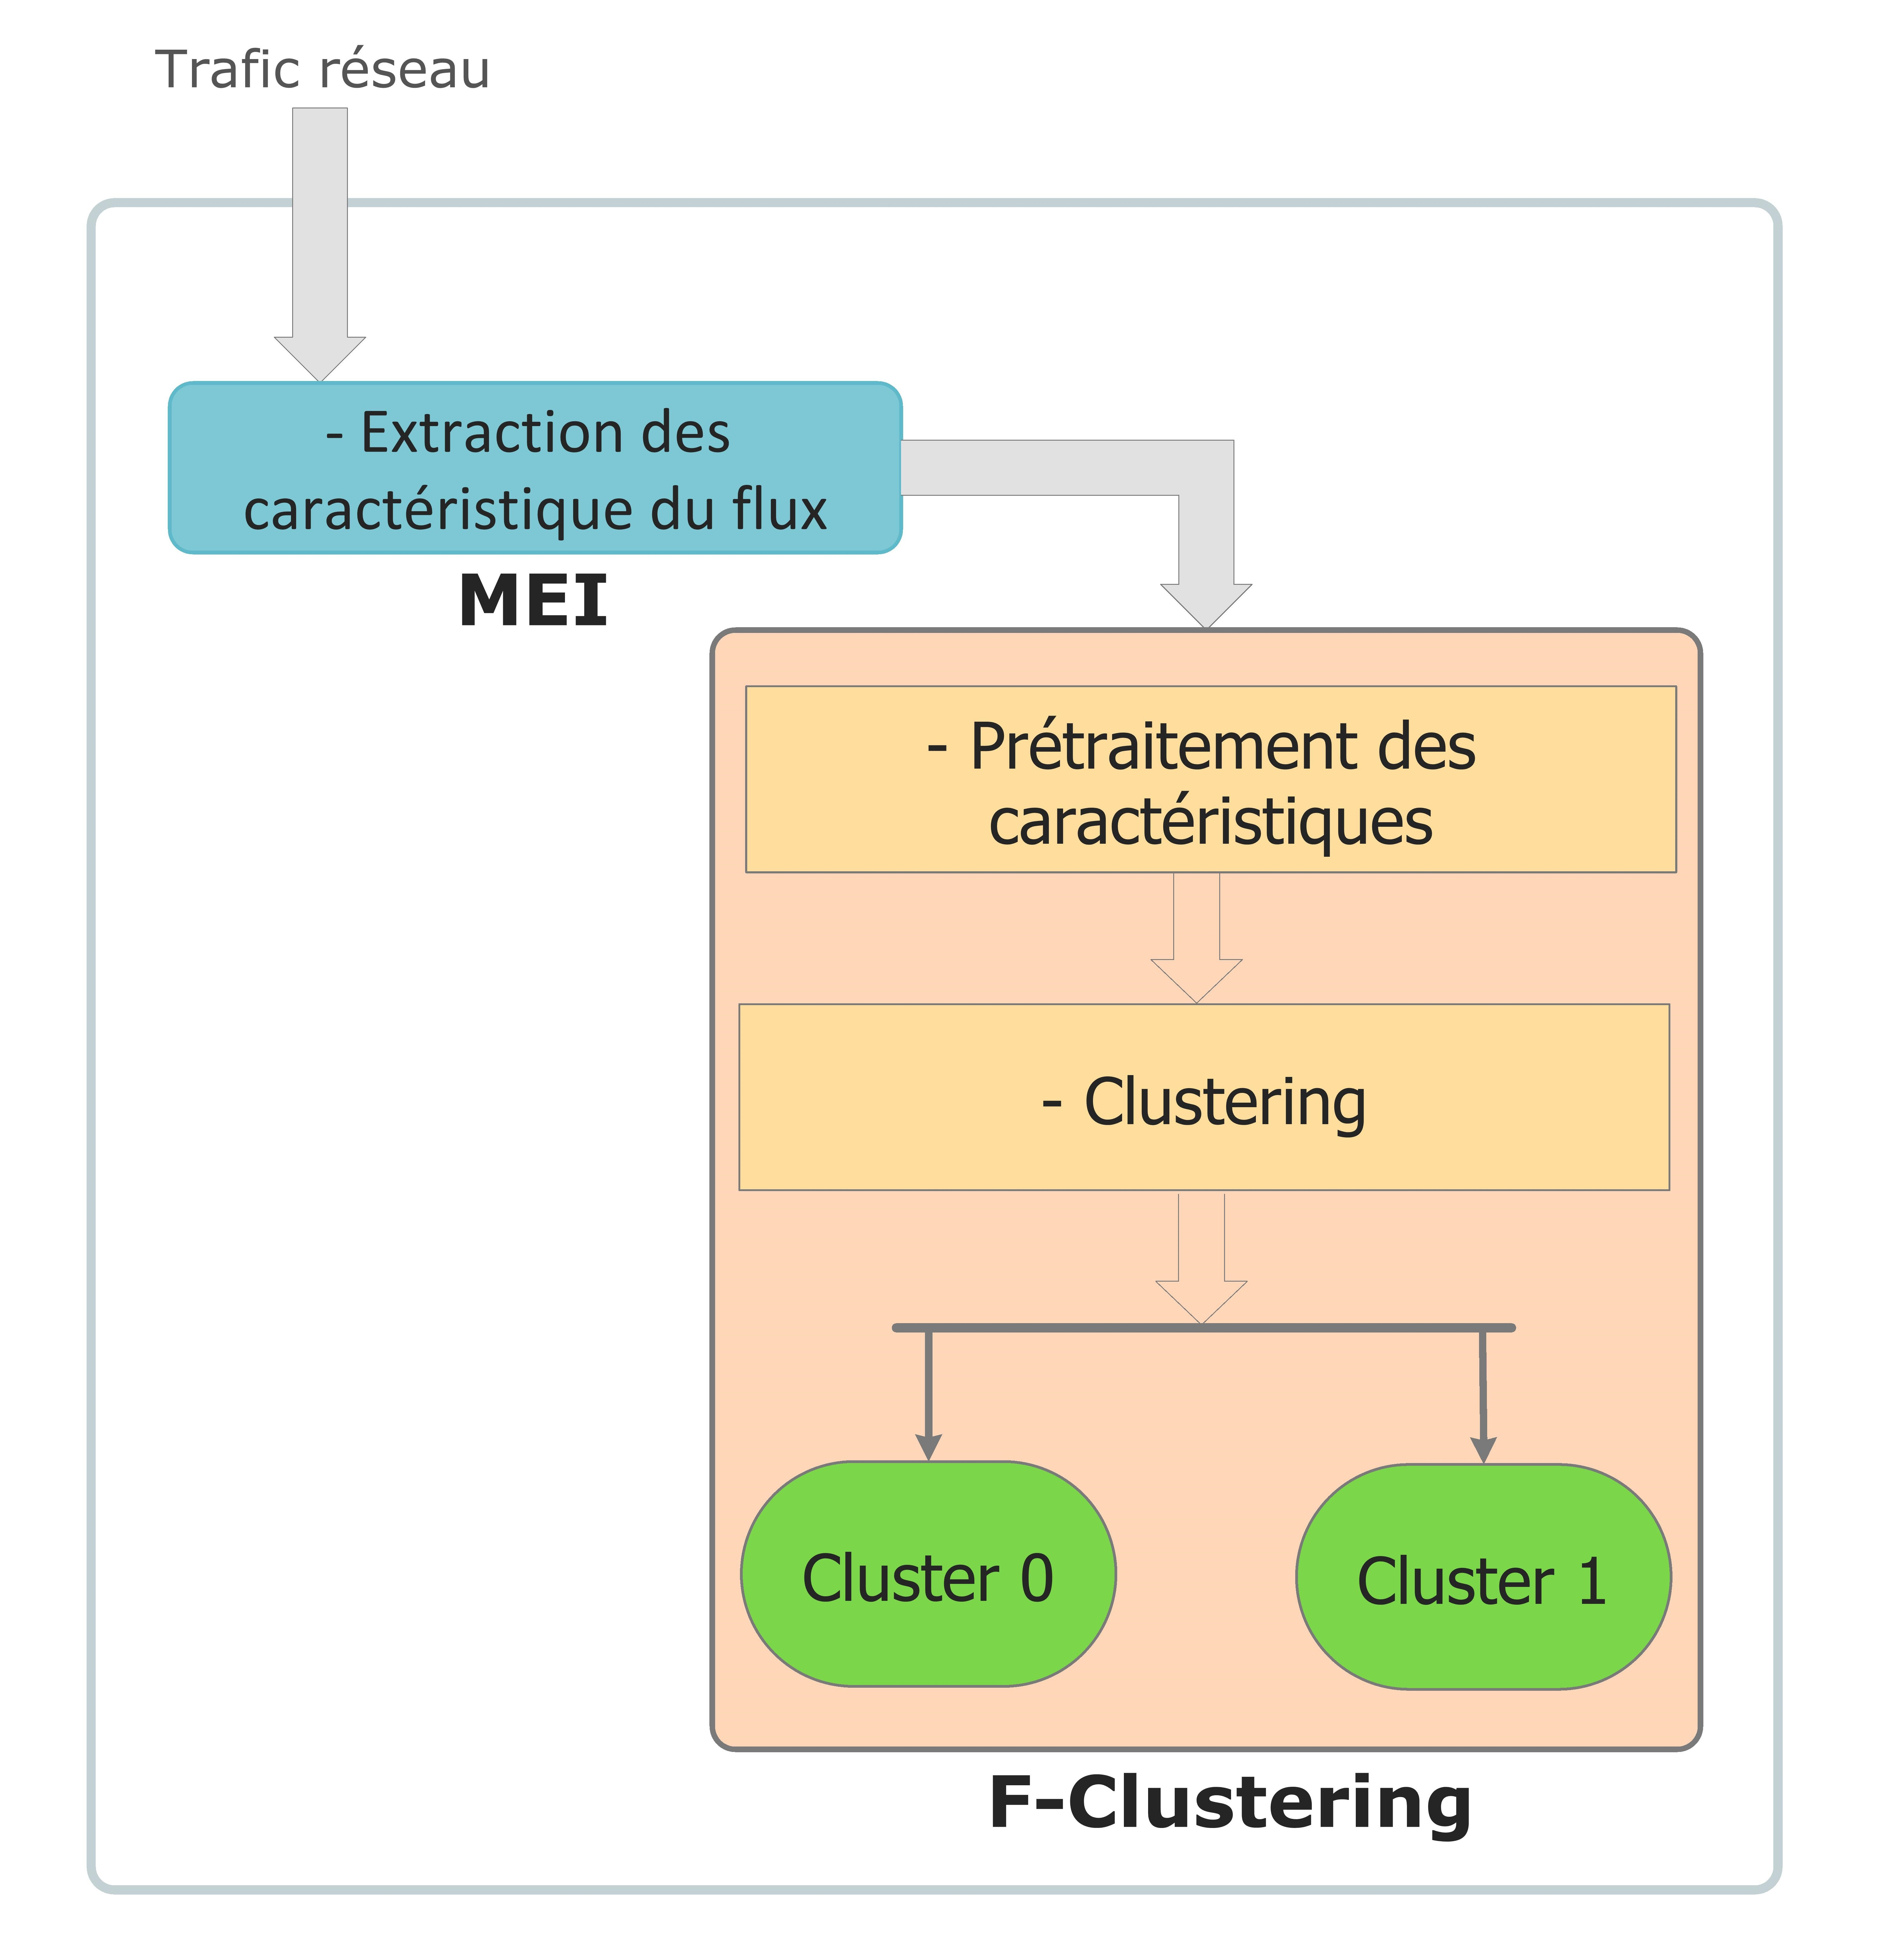
\includegraphics[width=\textwidth]{Figures/F-DoS}
\label{fig:rDoS}
\end{minipage}
\begin{minipage}[b]{.45\textwidth}
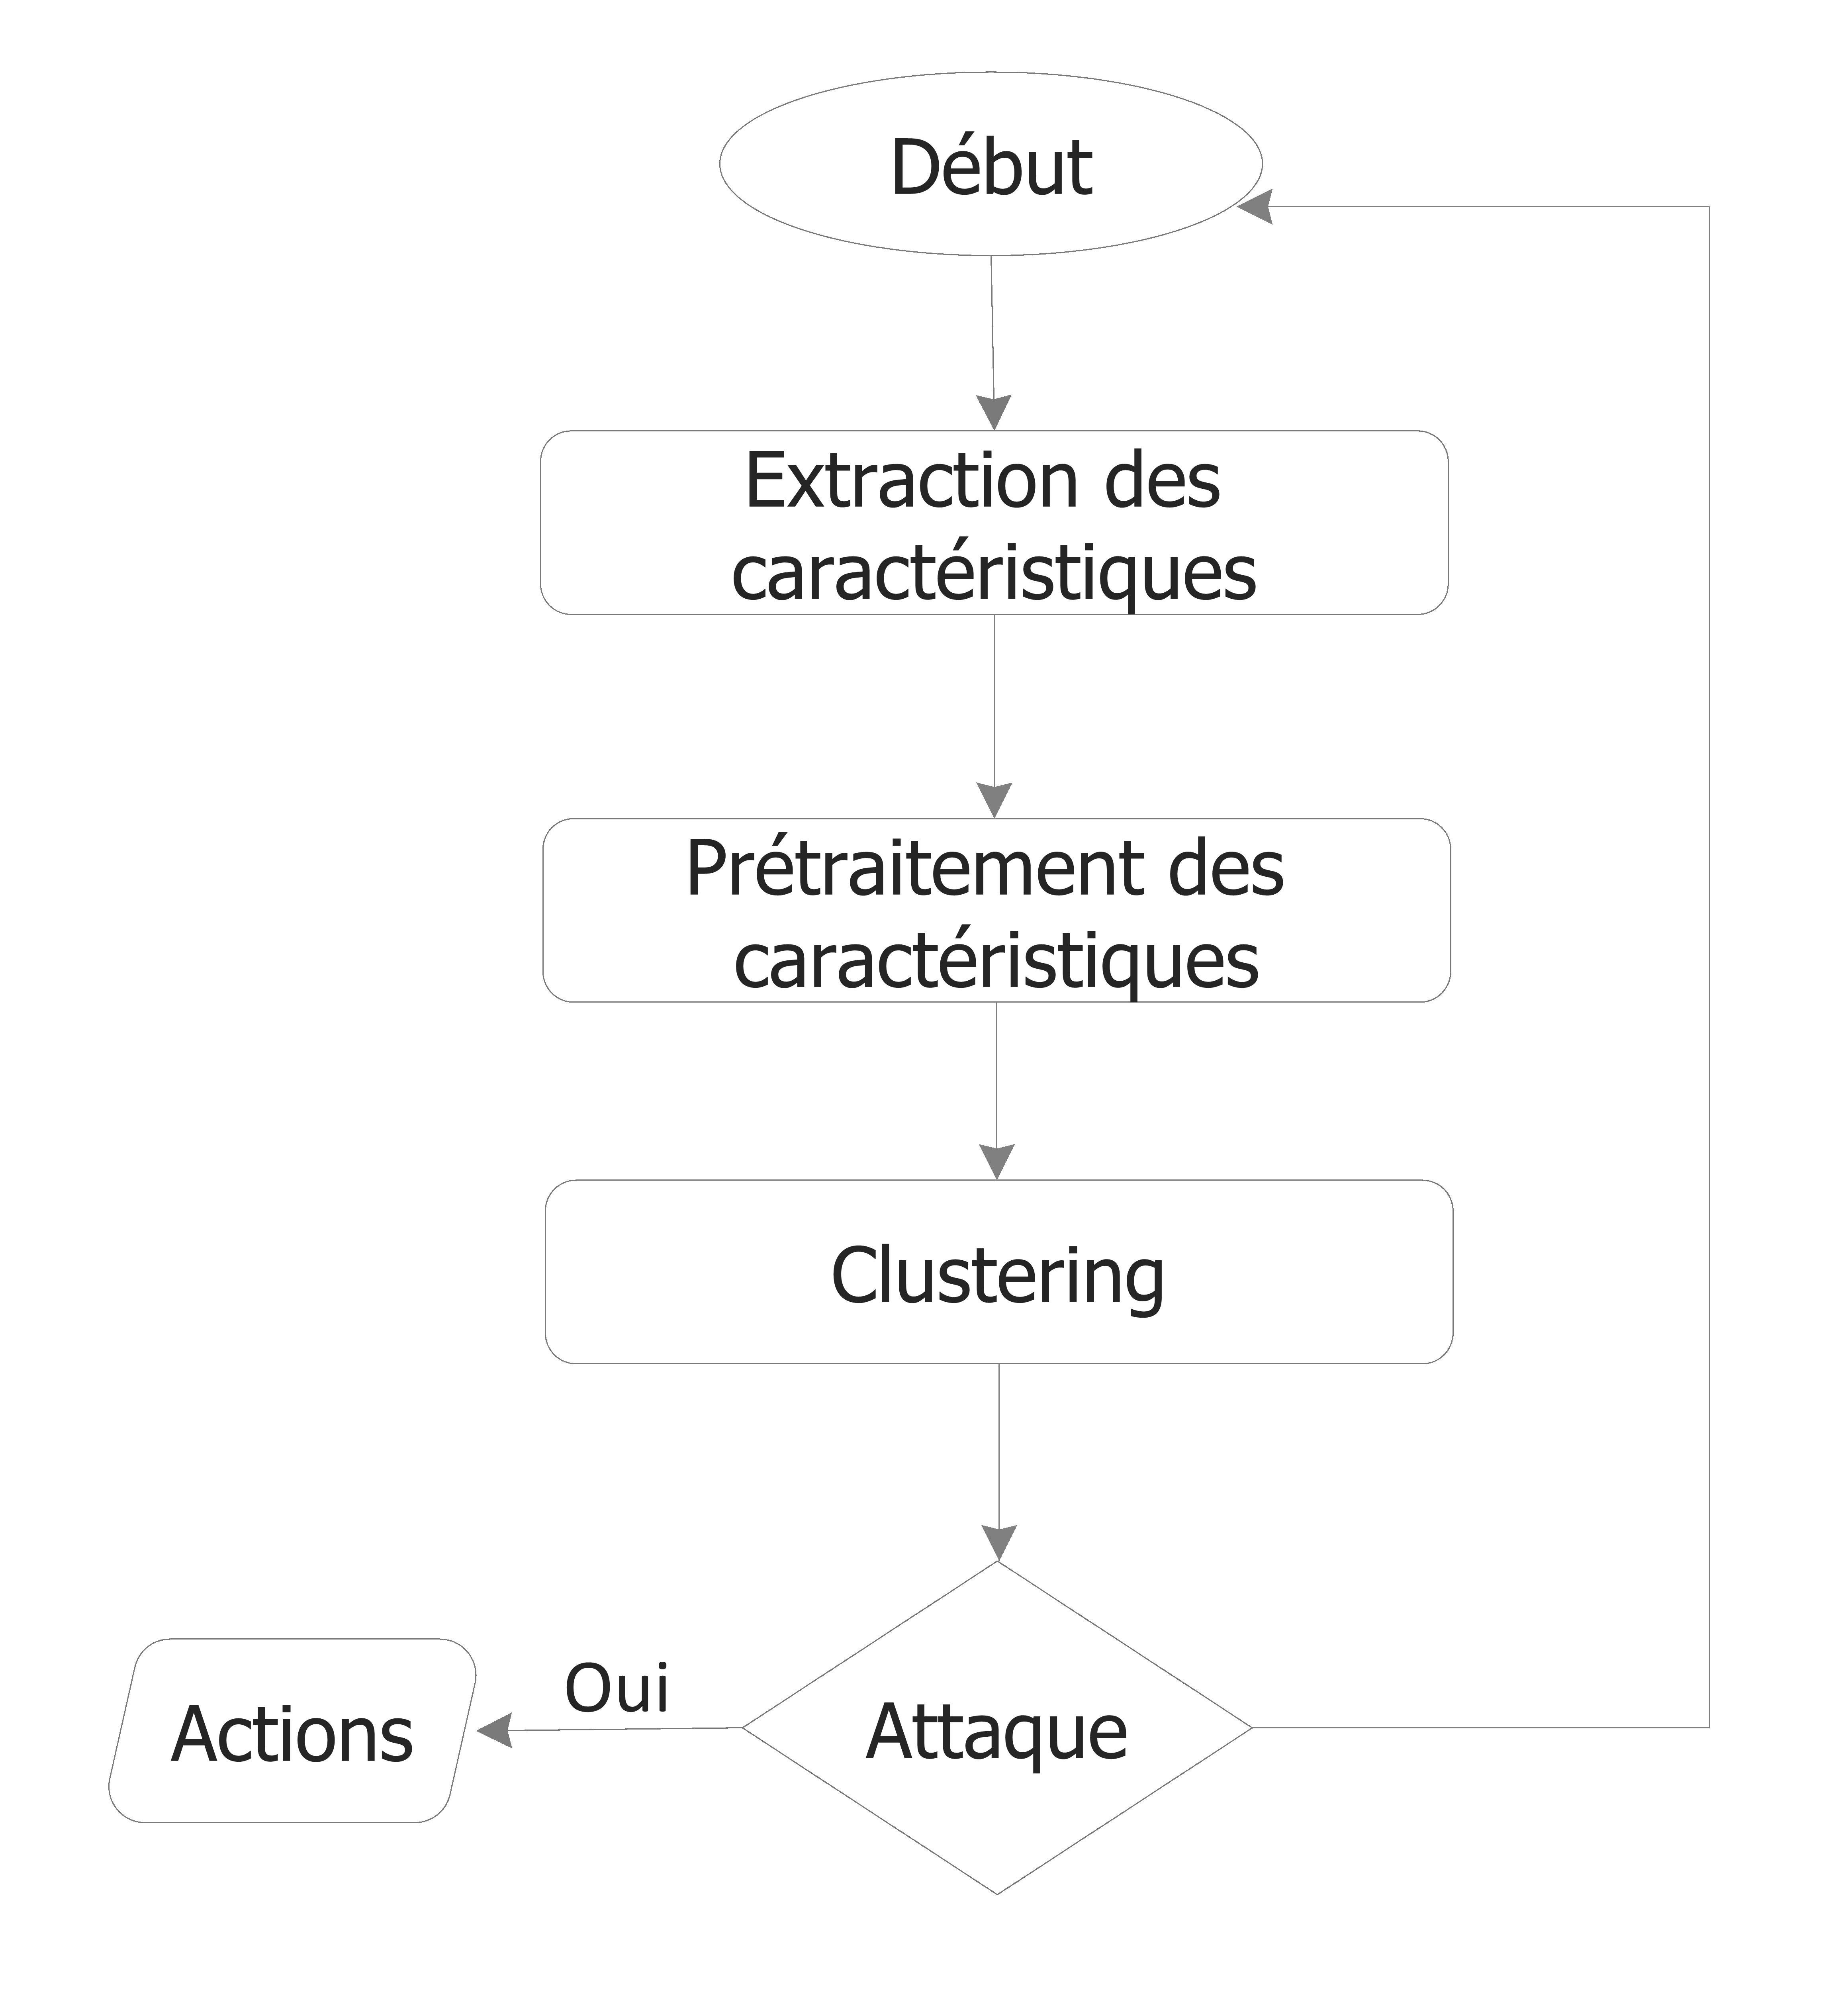
\includegraphics[width=\textwidth]{Figures/Diagramme}
\label{fig:rDoS}
\end{minipage}
\decoRule
\caption{Architecture et fonctionnemnt de F-DoS}
\end{figure}

\newpage
\subsection{Module MEI}
Le role principale de ce module est l'extractions d'information de flux de données. Mais pour ce faire, ce module doit assurer trois fonctions: l'écoute passive, l'analyse et l'ectraction. Ce module à un port didié à l'écoute, qui est toujours actif pour recevoir une copie de chaque paquet à l'aide de la téchnique de mise en miroir \textit{Port Miroring}. L'ensemble des paquets capturés est envoyé par la suite à l'analyseur. L'analyse des paquets n'est pas une fonction simple, elle doit être efféctuée soigneusement, si on analyse mal les paquets on risque de fausser le résultat de détection. Cette fonction est compliqué on raison que, l'analyseur recoit tous les paquets qui circulent dans le réseau, et on a dis précédemant qu'on s'intéresse au informations des flux de donnée, un flux est un ensemble de paquets qui on le même \textit{Paquet Header}(c-a-d même addresse source, addresse distination, port, ...etc). Donc l'analyseur doit filtrer les paquet; éliminer les paquets de contrôle, de solicitation, et tout autre paquet non intéréssant. Les paquet réstant sont ensuite regrouper en flux pour pouvoir ainsi exécuter la dernière fonction qui est l'éxtraction des caractéristiques. On parlera plus sur cet ensemble de caractéristiques et on justifiera le choix de chaqune dans la section ***.

\subsection{Module F-Clustering}
L'object de notre travail est de proposer une approche ce Clustering pour la détéction des attaques DoS. On s'est penché vers le K-Means, nous l'avons amélioré et adapté à notre utilisation pour construire notre modèle intelligent qui est le ceur de ce module. Ce module prend en entrée le vecteur de caractéristiques construit par le module MEI, et d'aprés ses préconaissance, et attribut le flux reçu a un des clusters préexistants. Si le flux est groupé dans le cluter des flux malin on dit qu'une attaque DoS (RDoS ou UDP-Flooding), on peut aisni lancer une alerte et c'est au administrateur réseau de prendre action.

\section{Construction du module F-Clustering}
Pour contruire ce module nous avons suivis les étapes du processus KDD décrites dans la section \ref{KDD}:
\begin{itemize}
\item[-] Préparation des données: première étapes du processus, où on parlera de notre source données et les différents opération effectuées sur ces données pour les preparer à la deuxième phase du processus. 
\item[-] Recherche du modèle: le modèle adopté est un modèle d'apprentissage non-supervisée, utilisant une approche de Clustering, qui va être trainer sur le données collectées dans la phase précendete.
\item[-] Évalutation du modèle: on ferra l'évaluation du modèle dans le chapitre \ref{Chapter5}.
\end{itemize}

\subsection{Préparation des données}
\subsubsection{DataSet : }
Comme source de données, nous avons exploité le dataset \textbf{ CICDDoS 2019}[\citep{18}]. CICDDoS2019 contient des flux bénigs et des attaques Ddos les plus courantes, qui ressemblent aux vraies données du monde réel. Ce dataset contient différentes attaques DoS modernes réfelectives telles que Portmap, Netbios, LDAP, UDP, TFTP, NTP. La période de capture a commencé le 12 janvier à 10 h 30 et s’est terminée à 17 h 15. Des attaques ont par la suite été exécutées au cours de cette période. \\

CICDDoS2019 formé de plusieurs fichier, chacun propres à une attaque. Vu la taille énormes de ces fichiers, et pour raison de simplifier le travail et pouvoir simuler l'architecture générale de notre réseau, on s'est mis d'accord sur le choix d'un seul fichier qu'on travaillera sur. Le fichier qu'on a choisi est propre à l'attaque TFTP, on réfénrencera par le nom "D-TFTP.\\

D-TFTP contien **** lignes. 
